\section{Angle Uncertainty Related to Converters}
\label{sec:uncertainty}

\pgfplotsset{shhc/.style={
    axis lines=left, xmajorgrids=true, ymajorgrids=true, grid style={gray!10},
    label style={font=\footnotesize}, tick label style={font=\footnotesize},
    every axis plot/.append style={line width=0.6pt, mark size=1.5pt, black},
    legend style={draw=none, font=\scriptsize, legend columns=-1, at={(0.5,1.02)}, anchor=south},
    legend cell align=left},
    iec/.style={gray!60, line width=1.2pt, mark=none},
    sbase/.style={solid, mark=*},
    sbank/.style={densely dashed, mark=o},
    scable/.style={densely dotted, mark=square},
    scablec/.style={dashdotted, mark=triangle}}

This section addresses the uncertainty of harmonic current phasors, especially phase angles, related to the typical industrial load with a 6-pulse line-commutated converter as shown in Fig. \ref{fig:topo_indust_LCC}.
% The Monte Carlo simulation is applied to the steady-state harmonic state-space model of the converter to assess the uncertainty propagation from key circuit parameters to harmonic phase angles.
First, a steady-state harmonic state-space model of the line-commutated converter is established, which captures the mutual coupling among the harmonic phasors and their dependence on key passive parameters.
% namely the commutation inductance $L_{ac}$ on the ac side and the smoothing inductance $L_{dc}$ on the dc side.
Then, the parameterized model is integrated into a stochastic assessment framework. The key parameters are modeled as random variables with realistic bounds. Monte Carlo simulation is applied to generate probability distributions of harmonic phasors.
% Finally, the marginal probability density functions are fitted using the best-fit method, and the Gaussian copula correlation matrix of harmonic phase angles is obtained to indicate the inter-harmonic correlation.
Finally, the Gaussian copula correlation matrix of harmonic phase angles is obtained to indicate the inter-harmonic correlation, and the shared probability density function is obtained.

\begin{figure}[!t]
\centering
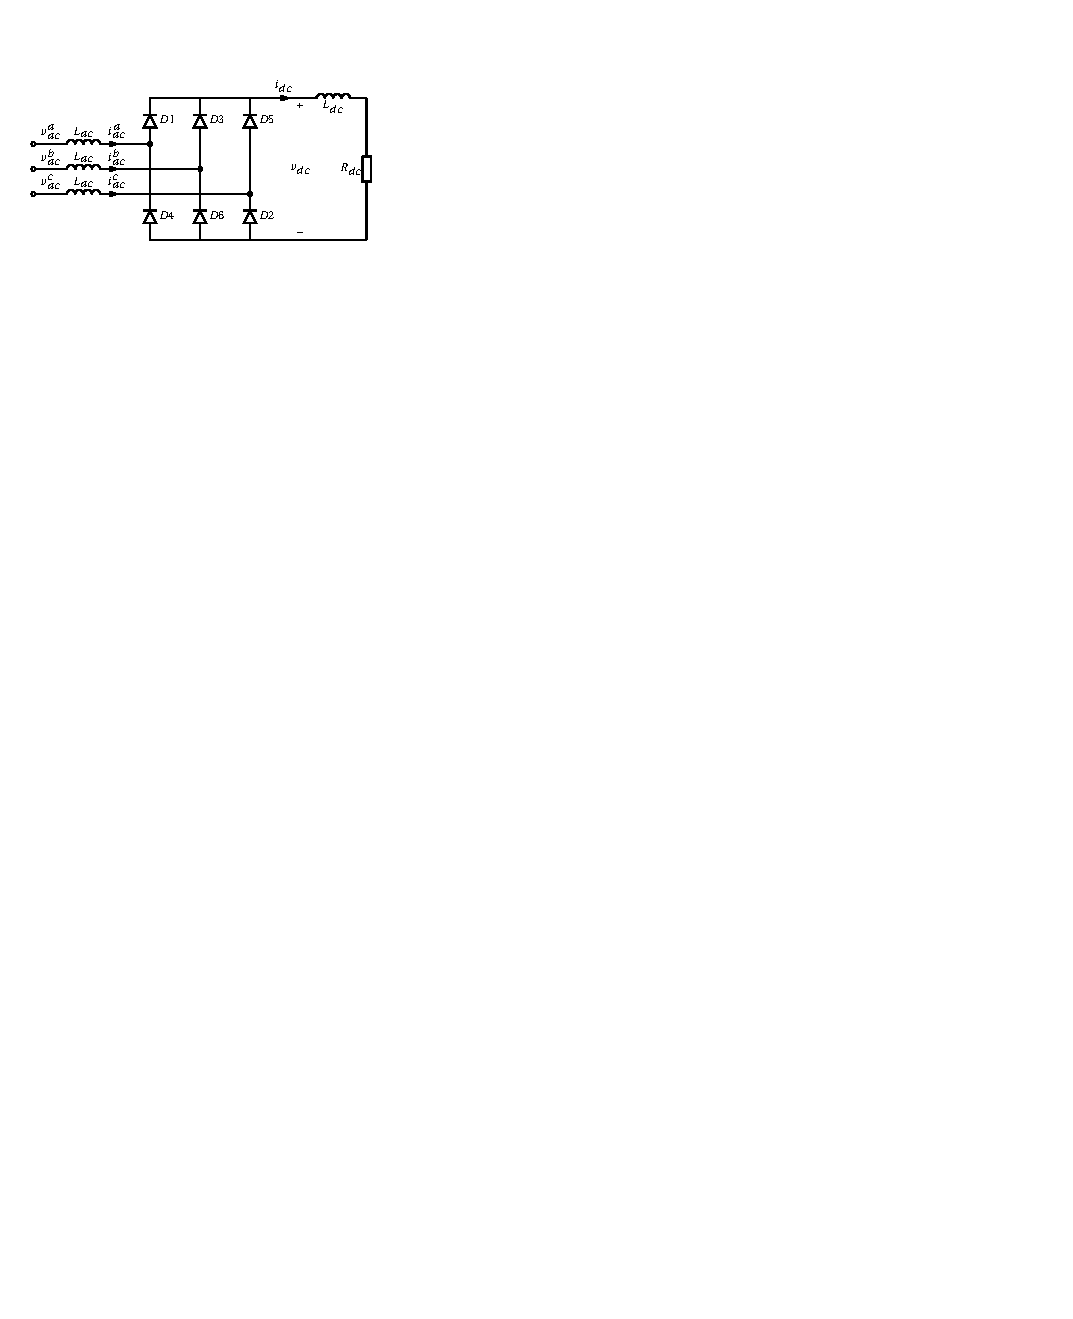
\includegraphics[width=0.6\columnwidth]{figures/topo_indust_LCC.pdf}
\caption{6-pulse line-commutated converter with ac-side commutation inductance~$L_{ac}$, dc-side smoothing inductance~$L_{dc}$ and dc load.}
\label{fig:topo_indust_LCC} 
\end{figure}

\subsection{Steady-State Harmonic Model} 
% Internal frequency coupling is the key feature of converter-generated harmonics, which decide the recombination of harmonic phasors. Therefore, the accurate harmonic state-space model is built here to capture the nature commutation and harmonic coupling of line-commutated converter.

The steady-state harmonic state-space model is used here to accurately capture the nature commutation and internal harmonic coupling of the line-commutated converter. The line-commutated converter periodically operates with sequential switching states, including 6 conducting states and 6 commutation states per fundamental period. Each state can be described by differential equations with time-varying coefficients that represent topology variations. The state equations for any switching state can be expressed as,
\begin{IEEEeqnarray}{l}
    (S_{dc} L_{ac} + L_{dc}) \frac{di_{dc}}{dt} = \nonumber \\
    S_{dc,ac}^{a} v_{ac}^a + S_{dc,ac}^{b} v_{ac}^b + S_{dc,ac}^{c} v_{ac}^c - R_{dc} i_{dc}, \label{eq:idc_t} \\
    % L_{ac} \frac{di_{ac}^a}{dt} - S_{dc,ac}^{a} L_{ac} \frac{di_{dc}}{dt} = \nonumber \\ S_{ac}^{a,a} v_{ac}^a + S_{ac}^{a,b} v_{ac}^b + S_{ac}^{a,c} v_{ac}^c, \label{eq:iac_t} \\
    L_{ac} \frac{di_{ac}^i}{dt} - S_{dc,ac}^{i} L_{ac} \frac{di_{dc}}{dt} = \nonumber \\ S_{ac}^{i,a} v_{ac}^a + S_{ac}^{i,b} v_{ac}^b + S_{ac}^{i,c} v_{ac}^c, \label{eq:iac_t}
\end{IEEEeqnarray}
where $v_{ac}^{i}$ and $i_{ac}^{i}$ denote ac-side voltage and current, $v_{dc}$ and $i_{dc}$ are dc-side voltage and current, the superscript $i,j \in \{a, b, c\}$ represents the three phases, $S_{dc,ac}^{i}(t)$, $S_{dc}(t)$, and $S_{ac}^{i,j}(t)$ are the piecewise switching functions reflecting the topology states.

The periodic equations in time-domain can be transformed into the harmonic state-space model in harmonic-domain through three operations: (i) Fourier series expansion of state variables $x(t) \leftrightarrow \sum_{h=-N_h}^{N_h} X_h e^{jh\omega_1 t}$ with truncated order $N_h$, (ii) frequency-domain differentiation $dx/dt \leftrightarrow \mathbf{Z}_{\Omega}\mathbf{X}$ where $\mathbf{Z}_{\Omega} = j\omega_1 \cdot \text{diag}(h)$, and (iii) Toeplitz convolution matrices representing time-domain multiplication: $y(t) = S(t)x(t) \leftrightarrow \mathbf{Y} = \mathbf{S}_{conv}\mathbf{X}$. The resulting unified system relates current harmonics $\mathbf{I} = [\mathbf{I}_{ac}^a, \mathbf{I}_{ac}^b, \mathbf{I}_{ac}^c]^T$ to voltage harmonics $\mathbf{U} = [\mathbf{V}_{ac}^a, \mathbf{V}_{ac}^b, \mathbf{V}_{ac}^c]^T$ through:

\begin{equation}
\mathbf{A}\mathbf{I} = \mathbf{B}\mathbf{U},
\label{eq:HSS}
\end{equation}
where matrices $\mathbf{A}$ and $\mathbf{B}$ contain Toeplitz convolution structures that explicitly capture frequency coupling. The model is parameterized by commutation overlap angle $\mu$, and the circuit inductances ($L_{ac}$, $L_{dc}$), providing a foundation for subsequent Monte Carlo simulation and uncertainty quantification.

\subsection{Methodology for Uncertainty Quantification}
In the planning stage, the uncertainty on key parameters comes from limited knowledge about the future integrated device, as well as manufacturing tolerances and operational variances. Therefore, inductance parameters $L_{ac}$ and $L_{dc}$ are modeled as random variables, and Monte Carlo simulation is used to assess the propagation of uncertainty.

\subsubsection{Realistic Parameter Distribution}
The uncertainties on $L_{ac}$ and $L_{dc}$ are modeled using truncated normal distributions:
\begin{equation}
L_{ac} \sim \mathcal{N}_{\text{trunc}}(\mu_{L_{ac}}, \sigma_{L_{ac}}^2, L_{ac,\min}, L_{ac,\max})
\label{truncated_normal_lac}
\end{equation}
\begin{equation}
L_{dc} \sim \mathcal{N}_{\text{trunc}}(\mu_{L_{dc}}, \sigma_{L_{dc}}^2, L_{dc,\min}, L_{dc,\max})
\label{truncated_normal_ldc}
\end{equation}
which are constrained within physically realistic bounds determined by engineering trade-offs at the industrial load design stage. For ac inductance $L_{ac}$, the upper bound $L_{ac,\max}$ is limited by the acceptable commutation angle and voltage drop, while the lower bound $L_{ac,\min}$ ensures adequate harmonic suppression and safe short-circuit current. For dc inductance $L_{dc}$, the upper bound $L_{dc,\max}$ is limited by dynamic response and size, while the lower bound $L_{dc,\min}$ ensures dc ripple to be within the specifications of power quality. The truncated normal distribution enforces physical bounds while maintaining mathematical tractability for Monte Carlo propagation.

% \begin{itemize}
%     \item \textit{ac-side inductance $L_{ac}$:} The upper bound $L_{ac,\max}$ is limited by acceptable commutation angle and voltage drop, while the lower bound $L_{ac,\min}$ ensures adequate harmonic suppression and safe short-circuit current.
%     \item \textit{dc-side inductance $L_{dc}$:} The upper bound $L_{dc,\max}$ is limited by required dynamic response, size, and cost, while the lower bound $L_{dc,\min}$ ensures dc ripple stays within specifications to prevent equipment aging and process quality degradation.
% \end{itemize}

\subsubsection{Monte Carlo Simulation}
Monte Carlo simulation is then implemented, by which 5000 pairs of random samples $(L_{ac}, L_{dc})$ are generated using rejection sampling to meet the defined constraints. For each of the parameter samples, a harmonic state-space model is built and solved. The iterative process involves: (i) recalculating the commutation angle $\mathsf{\mu}$ based on the sample pair of parameters; (ii) reconstructing the time-periodic switching functions $S_{dc,ac}^{i}(t)$, $S_{dc}(t)$, and $S_{ac}^{i,j}(t)$ using the updated commutation angle; and (iii) numerically solving the harmonic state-space equations to extract and store the magnitudes and phase angles of the ac-side harmonics.
% \begin{itemize}
%     \item Recalculating the commutation angle $\mathsf{\mu}$ based on the sampled pair of parameters.
%     \item Reconstructing time-periodic switching functions $S_{dc,ac}^{i}(t)$, $S_{dc}(t)$, and $S_{ac}^{i,j}(t)$ based on the updated commutation angle.
%     % \item Reconstructing time-periodic switching functions $\mathbf{S}_{dc,ac,conv}^{i}$, $\mathbf{S}_{dc,conv}$, and $\mathbf{S}_{ac,conv}^{i,j}$ based on the updated commutation angle.
%     \item Numerically solving the harmonic state-space equations to extract and store the magnitudes and phase angles of the ac-side harmonic currents of interest.
% \end{itemize}

\subsection{Dependency Analysis and Probability Density Function}
A case study is conducted based on a representative 6-pulse line-commutated converter unit, with nominal capacity of 1.25 MW and nominal voltage of 380 V, which is connected to the 35 kV bus through a rectifier transformer with a ratio of 35 kV/400 V. 
For the ac-side commutation inductance, the truncation bounds are $L_{ac,\min} = 0.01$ mH and $L_{ac,\max} = 0.03$ mH, corresponding to transformer short-circuit voltage ranging from $U_k = 5\%$ to $15\%$. For the dc-side smoothing inductance, the truncation bounds are $L_{dc,\min} = 0.05$ mH and $L_{dc,\max} = 0.35$ mH.

Fig.\ref{fig:harmonic_phasors_CI_LacLdc} shows the resulting phasor distribution of each characteristic harmonic. In each harmonic phasor distribution plot, the black arrow represent the phasors with mean magnitude and mean phase angle, while the dark gray represent the phasors within the 95\% confidence intervals. The results indicate that (i) the harmonic phasors at different frequencies exhibit mutual dependency; (ii) harmonics at higher orders display progressively larger angle variations and uncertainties. 

% \begin{figure}[!t]
%     \centering
%     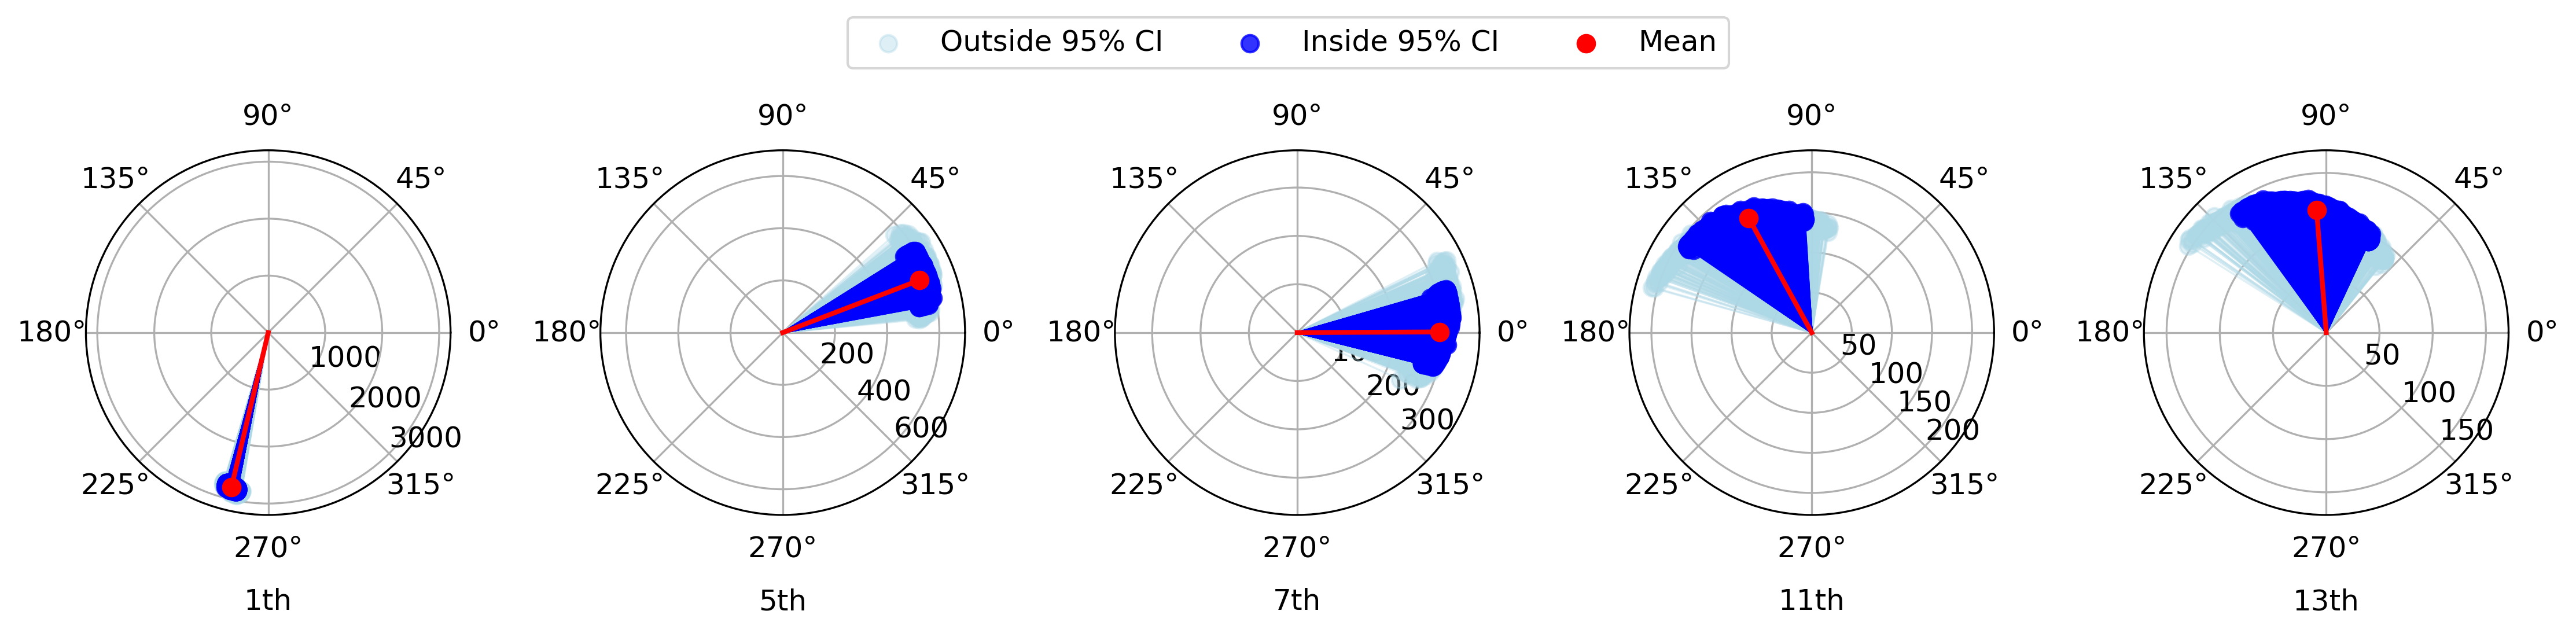
\includegraphics[width=\columnwidth]{figures/harmonic_phasors_CI_LacLdc.png}
%     \caption{Phasors of the characteristic harmonic currents of the converter of Fig.~\ref{fig:topo_indust_LCC} for 5000 Monte Carlo samples of~$L_{ac}$ and~$L_{dc}$: phasor with the mean magnitude and mean phase angle (red) and phasors within the 95\,\% confidence intervals (blue).}
%     \label{fig:harmonic_phasors_CI_LacLdc}
% \end{figure}

\usepgfplotslibrary{polar}
\providecommand{\Harmonic}{h}
\begin{figure*}[!t]
    \centering
    \pgfplotsset{phasorplot/.style={shhc, width=0.18\textwidth, ymin=0,
        xtick={0,90,180,270}, xticklabel={$\pgfmathprintnumber{\tick}^{\circ}$},
        yticklabel style={font=\tiny, anchor=north, inner sep=1.5pt, yshift=-2pt, /pgf/number format/1000 sep={}},
        every axis plot/.append style={line join=round}},
        outside/.style={only marks, mark=*, mark size=0.5pt, gray!35},
        inside/.style={only marks, mark=*, mark size=0.5pt, black!70},
        ci/.style={densely dashed, black, line width=0.5pt, mark=none},
        meanphasor/.style={-latex, black, line width=1pt, mark=none}}
    \subfloat[$\Harmonic = 1$]{%
    \begin{tikzpicture}
        \begin{polaraxis}[phasorplot, ymax=3200, ytick={1000,2000}, yticklabels={1k,2k}]
            \addplot[outside] table[x=angle, y=mag] {journals/shhc/data/phasor_ci/plot_outside_h1.dat};
            \addplot[inside] table[x=angle, y=mag] {journals/shhc/data/phasor_ci/plot_inside_h1.dat};
            \addplot[ci] table[x=angle, y=mag] {journals/shhc/data/phasor_ci/ci_h1.dat};
            \addplot[meanphasor] table[x=angle, y=mag] {journals/shhc/data/phasor_ci/mean_h1.dat};
        \end{polaraxis}
    \end{tikzpicture}}%
    \subfloat[$\Harmonic = 5$]{%
    \begin{tikzpicture}
        \begin{polaraxis}[phasorplot, ymax=700, ytick={300,600}]
            \addplot[outside] table[x=angle, y=mag] {journals/shhc/data/phasor_ci/plot_outside_h5.dat};
            \addplot[inside] table[x=angle, y=mag] {journals/shhc/data/phasor_ci/plot_inside_h5.dat};
            \addplot[ci] table[x=angle, y=mag] {journals/shhc/data/phasor_ci/ci_h5.dat};
            \addplot[meanphasor] table[x=angle, y=mag] {journals/shhc/data/phasor_ci/mean_h5.dat};
        \end{polaraxis}
    \end{tikzpicture}}%
    \subfloat[$\Harmonic = 7$]{%
    \begin{tikzpicture}
        \begin{polaraxis}[phasorplot, ymax=370, ytick={150,300}, yticklabels={150,}]
            \addplot[outside] table[x=angle, y=mag] {journals/shhc/data/phasor_ci/plot_outside_h7.dat};
            \addplot[inside] table[x=angle, y=mag] {journals/shhc/data/phasor_ci/plot_inside_h7.dat};
            \addplot[ci] table[x=angle, y=mag] {journals/shhc/data/phasor_ci/ci_h7.dat};
            \addplot[meanphasor] table[x=angle, y=mag] {journals/shhc/data/phasor_ci/mean_h7.dat};
        \end{polaraxis}
    \end{tikzpicture}}%
    \subfloat[$\Harmonic = 11$]{%
    \begin{tikzpicture}
        \begin{polaraxis}[phasorplot, ymax=230, ytick={100,200}]
            \addplot[outside] table[x=angle, y=mag] {journals/shhc/data/phasor_ci/plot_outside_h11.dat};
            \addplot[inside] table[x=angle, y=mag] {journals/shhc/data/phasor_ci/plot_inside_h11.dat};
            \addplot[ci] table[x=angle, y=mag] {journals/shhc/data/phasor_ci/ci_h11.dat};
            \addplot[meanphasor] table[x=angle, y=mag] {journals/shhc/data/phasor_ci/mean_h11.dat};
        \end{polaraxis}
    \end{tikzpicture}}%
    \subfloat[$\Harmonic = 13$]{%
    \begin{tikzpicture}
        \begin{polaraxis}[phasorplot, ymax=170, ytick={50,100}]
            \addplot[outside] table[x=angle, y=mag] {journals/shhc/data/phasor_ci/plot_outside_h13.dat};
            \addplot[inside] table[x=angle, y=mag] {journals/shhc/data/phasor_ci/plot_inside_h13.dat};
            \addplot[ci] table[x=angle, y=mag] {journals/shhc/data/phasor_ci/ci_h13.dat};
            \addplot[meanphasor] table[x=angle, y=mag] {journals/shhc/data/phasor_ci/mean_h13.dat};
        \end{polaraxis}
    \end{tikzpicture}}
    \caption{Phasors of characteristic harmonic currents, 1000 of the 5000 Monte Carlo samples, inside (dark gray) and outside (light gray) the 95\,\% confidence region of magnitude and phase angle (dashed), with the mean phasor (black arrow): (a) $\Harmonic = 1$; (b) $\Harmonic = 5$; (c) $\Harmonic = 7$; (d) $\Harmonic = 11$; (e) $\Harmonic = 13$.}
    \label{fig:harmonic_phasors_CI_LacLdc}
\end{figure*}

\subsubsection{Inter-Harmonic Dependency Analysis}
An important feature of the harmonics generated by the line-commutated converter is the inter-harmonic dependency due to frequency coupling, as indicated by the harmonic state-space model in ~\eqref{eq:HSS}. To characterize the dependencies among harmonic components, the correlation matrices with Kendall's Tau correlation coefficients are obtained.
% To assess this dependency, the correlation structure between different harmonic components is investigated. Correlation matrices, with Kendall's Tau correlation coefficients, are used to characterize the dependencies.
As shown by the phase angle correlation matrix $\mathbf{R}_{\text{phase}}$ in Fig.~\ref{fig:Correlation_Matrix_Copula}, phase angles have strong inter-harmonic dependency with the Gaussian copula parameters $\rho_{ij}^{Gauss} \geq 0.97$.
% indicating distinct characteristics in the inter-harmonic dependency structure for phase angles.

% \begin{figure}[!t]
%     \centering
%     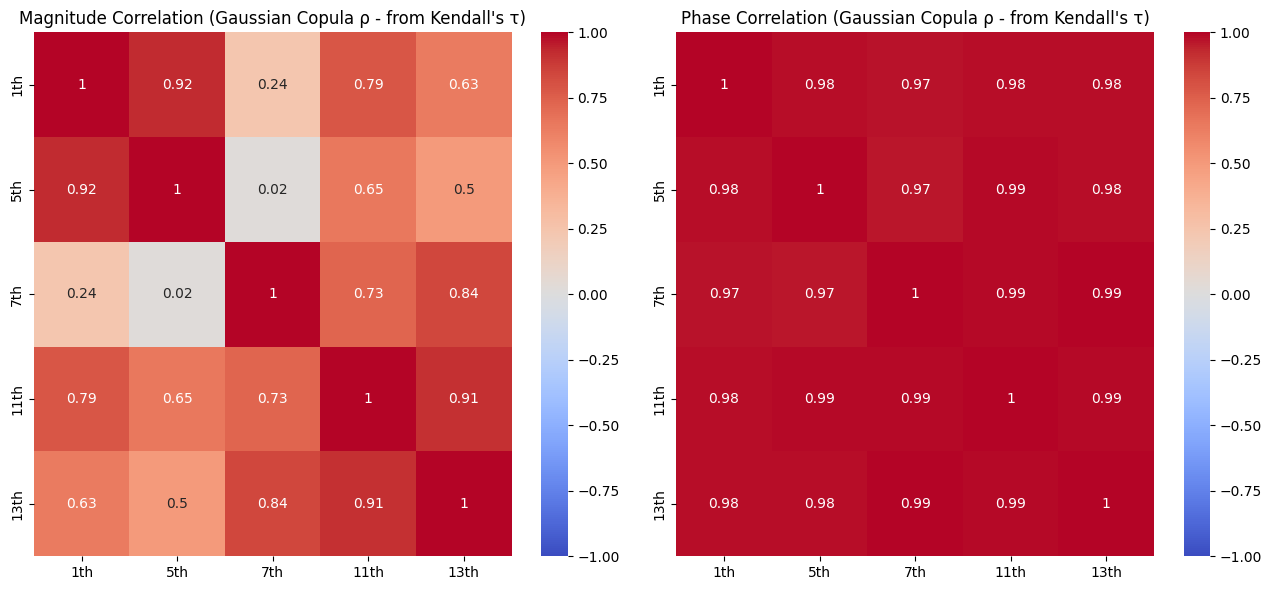
\includegraphics[width=\columnwidth]{figures/Correlation_Matrix_Copula.png}
%     \caption{Gaussian copula correlation matrices of the harmonic current magnitudes and of the harmonic current phase angles across the harmonic orders, from 5000 Monte Carlo samples of~$L_{ac}$ and~$L_{dc}$.}
%     \label{fig:Correlation_Matrix_Copula}
% \end{figure}

\providecommand{\Harmonic}{h}
\begin{figure}[!t]
    \centering
    \pgfplotsset{corrplot/.style={shhc, grid=none, scale only axis, width=3.2cm, height=3.2cm,
        xmin=-0.5, xmax=4.5, ymin=-0.5, ymax=4.5, y dir=reverse, axis on top,
        xtick={0,...,4}, ytick={0,...,4}, xticklabels={1,5,7,11,13}, yticklabels={1,5,7,11,13},
        tick style={draw=none}, xlabel={harmonic order $\Harmonic$},
        colormap={gray}{color=(white) color=(gray!70)}, point meta min=0, point meta max=1,
        nodes near coords={\pgfmathprintnumber[fixed, fixed zerofill, precision=2]{\pgfplotspointmeta}},
        every node near coord/.append style={font=\tiny, black, anchor=center}},
        corrcells/.style={matrix plot*, mesh/cols=5, point meta=explicit, draw=white, line width=0.4pt}}
    \subfloat[magnitude]{%
    \begin{tikzpicture}
        \begin{axis}[corrplot, ylabel={harmonic order $\Harmonic$}]
            \addplot[corrcells] table[x=col, y=row, meta=rho] {journals/shhc/data/copula_corr/corr_mag.dat};
        \end{axis}
    \end{tikzpicture}}%
    \subfloat[phase angle]{%
    \begin{tikzpicture}
        \begin{axis}[corrplot]
            \addplot[corrcells] table[x=col, y=row, meta=rho] {journals/shhc/data/copula_corr/corr_phase.dat};
        \end{axis}
    \end{tikzpicture}}
    \caption{Dependence between the harmonic currents of the industrial load, Gaussian copula correlation matrices with parameters $\rho_{ij}^{Gauss}$ obtained from Kendall's rank correlation~$\tau$ of 5000 Monte Carlo samples, darker cells for stronger correlation: (a) magnitudes; (b) phase angles.}
    \label{fig:Correlation_Matrix_Copula}
\end{figure}

% \subsubsection{Marginal Distribution Fitting}
% The marginal distributions of each harmonic component are modeled independently. The best-fit probability density function for each harmonic magnitude and phase angle is fitted to the data obtained from Monte Carlo simulation. The candidate distributions considered include Normal, Lognormal, Beta, Logistic and Exponential distributions.

% For each harmonic $h$, the marginal distribution $F_h(x_h)$ is estimated by fitting multiple parametric distributions and selecting the best-fit  distribution based on minimizing the root-mean-square error between the cumulative distribution functions simulated and fitted. The best-fit results are illustrated in Fig.\ref{fig:Bestfit_PDF}, showing the histograms and the fitted probability density functions of harmonic magnitudes and phase angles.

% Tables~\ref{tab:bestfit_phase} summarize the best-fit distributions and their estimated parameters for harmonic phase angles.
% \begin{table}[h] 
% \centering
% \caption{Best-Fit Distributions for Harmonic Phase Angles}
% \label{tab:bestfit_phase}
% \begin{tabular}{l l l l}
% \hline
% Order & distribution & error & parameters \\
% \hline
% 1st  & Beta    & $9.30 e^{-3}$ & $[ 10.8052, 20.2376, -107.9443, 13.0245]$ \\
% 5th  & Beta    & $1.97 e^{-3}$ & $[11.8144, 23.6725, -2.6825, 70.8689]$ \\
% 7th  & Beta    & $1.54 e^{-3}$ & $[ 9.7918, 18.8775, -29.9737, 88.2789]$ \\
% 11th & Beta    & $7.41 e^{-4}$ & $[ 12.4463, 22.1493, 59.5585, 164.3101]$ \\
% 13th & Beta    & $6.84 e^{-4}$ & $[ 10.4088, 17.2887, 29.4667, 172.4882]$ \\
% \hline
% \end{tabular}
% \end{table}

% The parameters of the Beta distribution are given as $[\alpha, \beta, \ell, \theta]$, where $\alpha$ and $\beta$ are the shape parameters, and $\ell$ and $\theta$ are the location and scale parameters, respectively.

% \begin{figure*}[h!]
%     \centering
%     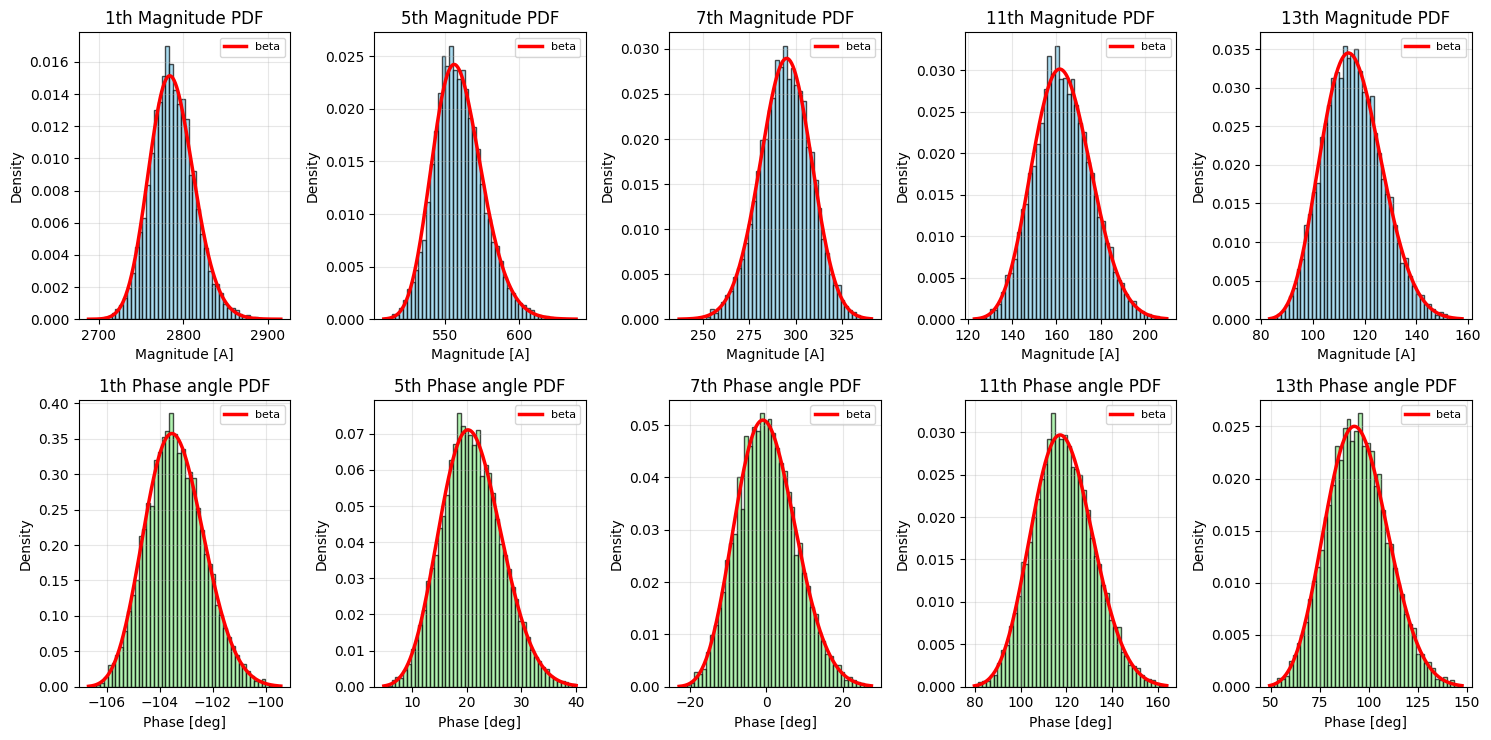
\includegraphics[width=0.8\textwidth]{figures/Bestfit_PDF.png}
%     \caption{Histograms of the harmonic current magnitudes and phase angles from 5000 Monte Carlo samples of~$L_{ac}$ and~$L_{dc}$, with the best-fit probability density functions of Table~\ref{tab:bestfit_phase}.}
%     \label{fig:Bestfit_PDF} 
% \end{figure*}

\subsubsection{Shared Beta Distribution for Phase Angles}
Since strong inter-harmonic dependencies are proved for phase angles, a shared Beta distribution is used to represent the normalized phase angle distributions across the harmonic orders. In this way, only two shape parameters, $\alpha$ and $\beta$, are estimated for all harmonics, while each harmonic retains its own location and scale parameters to capture the specific range of phase angles.

Firstly, a normalization procedure is applied to the unwrapped phase angle data of each harmonic to map them to the unit interval $[0,1]$. Let $\phi_h = \{\phi_{h,i}\}_{i=1}^{N}$ denote the unwrapped phase angle samples in degrees for harmonic $h \in \{1, 5, 7, 11, 13\}$, where unwrapping avoids discontinuities at $\pm 180^\circ$. For each harmonic, the observed min–max values are $v_{\min,h} = \min(\phi_h)$ and $v_{\max,h} = \max(\phi_h)$.
% \begin{equation}
% v_{\min,h} = \min(\phi_h), \qquad v_{\max,h} = \max(\phi_h).
% \end{equation}
The sampled data of each harmonic phase angle are then normalized to the unit interval via the min-max transformation:
\begin{equation}
u_{h,i} = \frac{\phi_{h,i} - v_{\min,h}}{v_{\max,h} - v_{\min,h}} \in (0,1).
\end{equation}

Secondly, all normalized samples from the five harmonics are pooled into a single dataset:
\begin{equation}
\mathcal{U} = \bigcup_{h \in \{1,5,7,11,13\}} \{u_{h,i}\}_{i=1}^{N}.
\end{equation}

A single Beta distribution with estimated shape parameters $\hat{\alpha}$ and $\hat{\beta}$ is fitted to $\mathcal{U}$ via maximum likelihood estimation, with location and scale fixed to the standard interval $[0,1]$:
\begin{equation}
u \sim \mathrm{Beta}(\hat{\alpha}, \hat{\beta}).
\end{equation}

The results of the fitted parameters are $\hat{\alpha} = 4.0414$, $\hat{\beta} = 4.7762$. The Beta probability density function is given by:
\begin{equation}
f_{\mathrm{Beta}}(u; \hat{\alpha}, \hat{\beta}) = \frac{u^{\hat{\alpha}-1}(1-u)^{\hat{\beta}-1}}{\int_0^1 t^{\hat{\alpha}-1}(1-t)^{\hat{\beta}-1}\,dt}, \quad u \in (0,1).
\end{equation}

Thirdly, the fitted shared Beta distribution is transformed back to each harmonic's phase angle scale to assess the goodness-of-fit. For each harmonic $h$, the denormalization is performed as:
\begin{equation}
\label{eq:beta_denorm}
f_{\phi_h}(\phi) = \frac{1}{v_{\max,h} - v_{\min,h}} \, f_{\mathrm{Beta}}\!\left(\frac{\phi - v_{\min,h}}{v_{\max,h} - v_{\min,h}}; \hat{\alpha}, \hat{\beta}\right),
\end{equation}
where $\phi\in [v_{\min,h}, v_{\max,h}]$ is the original phase angle range for harmonic $h$.

Table~\ref{tab:beta_phase_params} lists the shared shape parameters, harmonic-specific locations $v_{\min,h}$ and scales $(v_{\max,h} - v_{\min,h})$, and the root-mean-square errors between the empirical histograms from the Monte Carlo simulation and the denormalized Beta probability density functions.
% The goodness-of-fit of the shared Beta distribution model is evaluated for each harmonic phase angle by comparing the denormalized Beta probability density function against the empirical histograms from Monte Carlo simulation. The root-mean-square error is computed between the empirical histogram and the denormalized Beta probability density function, with the results summarized in last column of Table~\ref{tab:beta_phase_params}.
The comparison plots between the empirical histograms and the denormalized shared Beta probability density functions for each harmonic phase angle are shown in Fig.~\ref{fig:Shared_Beta_Fit}. Both the visual comparison and the low root-mean-square errors indicate a good fit of the shared Beta distribution to the simulated data across all harmonics.

\begin{table}[!t]
    \centering
    \caption{Shared Beta distribution parameters and fit quality for harmonic phase angles}
    \label{tab:beta_phase_params}
    \scriptsize
    \begin{tabular}{l c c c c}
    Order & $v_{\min}$ [deg] & $v_{\max}$ [deg] & $v_{\max} - v_{\min}$ [deg] & error \\
    \hline
    1st  & $-106.70$ & $-99.43$   & 7.27   & 0.0226 \\
    5th  & 4.75      & 40.05      & 35.30  & 0.0037 \\
    7th  & $-22.77$  & 27.51      & 50.28  & 0.0029 \\
    11th & 79.69     & 164.01     & 84.32  & 0.0014 \\
    13th & 49.38     & 147.67     & 98.29  & 0.0011 \\
    \end{tabular}
    
    \vspace{2pt}
    \parbox{\columnwidth}{\scriptsize All harmonics share the same shape parameters ($\hat{\alpha} = 4.041$, $\hat{\beta} = 4.776$).\\
    Location parameters $v_{\min}$ and scale parameter $(v_{\max} - v_{\min})$ are harmonic-specific.}
    % \multicolumn{7}{l}{\footnotesize Note: All harmonics share the same shape parameters ($\hat{\alpha} = 4.041$, $\hat{\beta} = 4.776$).} \\
    % \multicolumn{7}{l}{\footnotesize Location parameter $v_{\min}$ and scale parameter $(v_{\max} - v_{\min})$ are harmonic-specific.} \\
\end{table}

% \begin{figure}[!b]
%     \centering
%     % 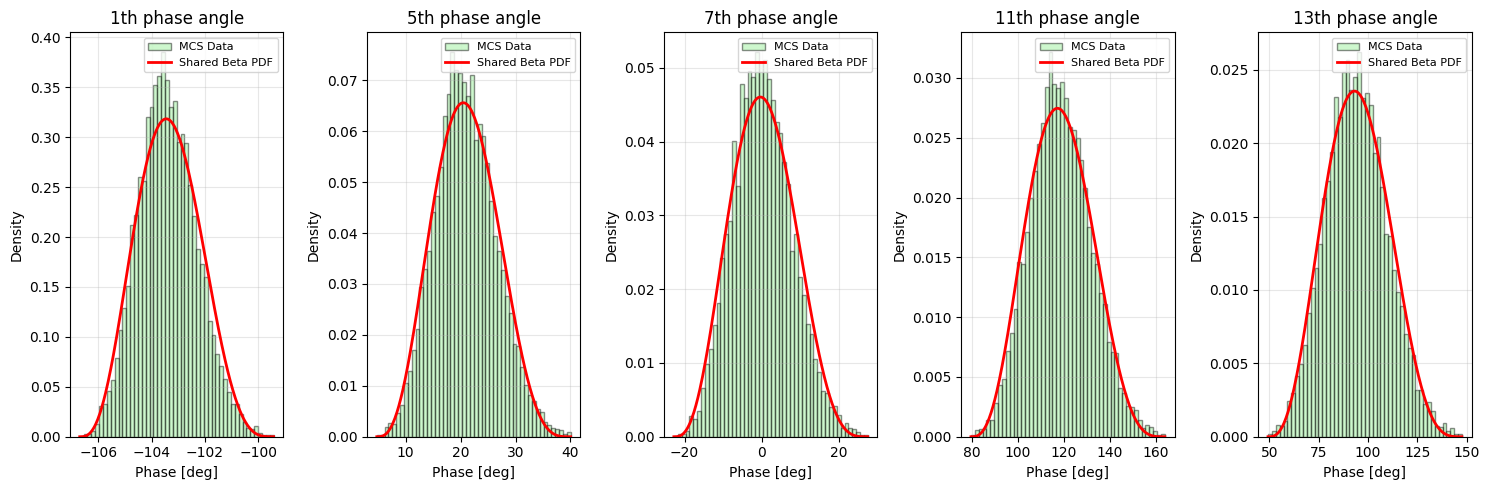
\includegraphics[width=0.8\textwidth]{figures/Shared_Beta_Fit.png}
%     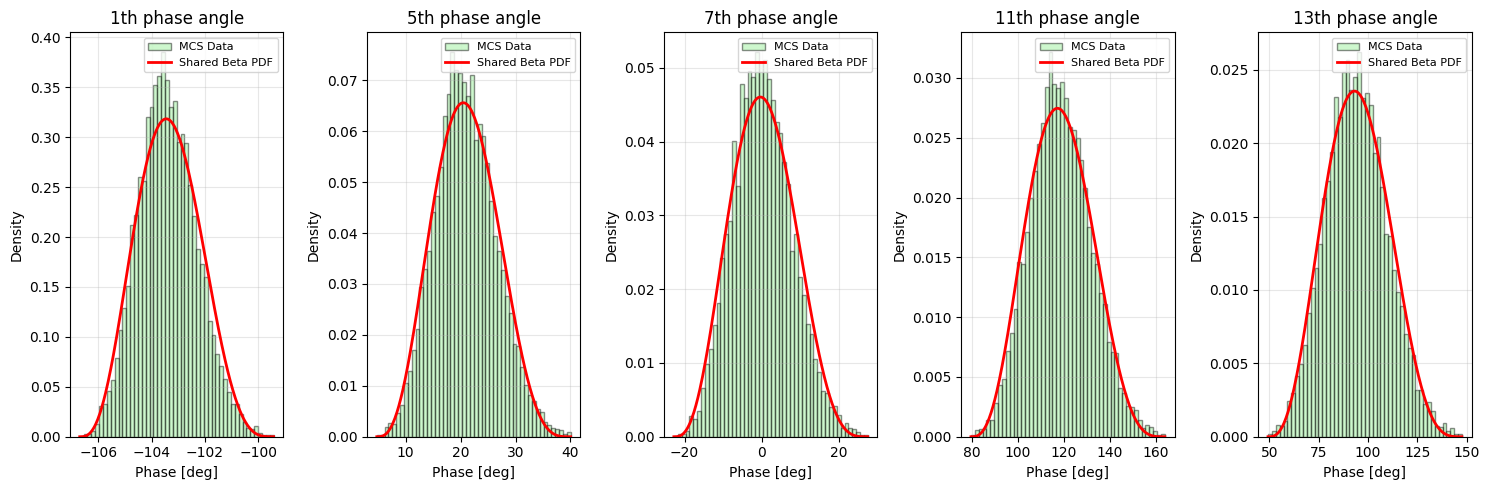
\includegraphics[width=\columnwidth]{figures/Shared_Beta_Fit.png}
%     \caption{Histograms of the harmonic current phase angles from 5000 Monte Carlo samples of~$L_{ac}$ and~$L_{dc}$, and the denormalized shared Beta probability density functions with parameters listed in Table~\ref{tab:beta_phase_params}.}
%     \label{fig:Shared_Beta_Fit} 
% \end{figure}

\begin{figure*}[!t]
    \centering
    \pgfplotsset{phaseplot/.style={shhc, width=0.205\textwidth, height=3cm, ymin=0,
        xlabel={phase [deg]}, scaled y ticks=false, yticklabel style={/pgf/number format/fixed},
        every axis plot/.append style={mark=none}},
        mcs/.style={ybar interval, fill=gray!30, draw=gray!70, line width=0.2pt},
        beta/.style={solid, black, line width=0.9pt}}
    \subfloat[$h = 1$]{%
    \begin{tikzpicture}
        \begin{axis}[phaseplot, xtick={-106,-103,-100}, ylabel={PDF [1/deg]}]
            \addplot[mcs] table[x=x, y=density] {journals/shhc/data/shared_beta_phase/hist_interval_h1.dat};
            \addplot[beta] table[x=x, y=pdf] {journals/shhc/data/shared_beta_phase/pdf_h1.dat};
        \end{axis}
    \end{tikzpicture}}%
    \subfloat[$h = 5$]{%
    \begin{tikzpicture}
        \begin{axis}[phaseplot, xtick={10,20,30}]
            \addplot[mcs] table[x=x, y=density] {journals/shhc/data/shared_beta_phase/hist_interval_h5.dat};
            \addplot[beta] table[x=x, y=pdf] {journals/shhc/data/shared_beta_phase/pdf_h5.dat};
        \end{axis}
    \end{tikzpicture}}%
    \subfloat[$h = 7$]{%
    \begin{tikzpicture}
        \begin{axis}[phaseplot, xtick={-20,0,20}]
            \addplot[mcs] table[x=x, y=density] {journals/shhc/data/shared_beta_phase/hist_interval_h7.dat};
            \addplot[beta] table[x=x, y=pdf] {journals/shhc/data/shared_beta_phase/pdf_h7.dat};
        \end{axis}
    \end{tikzpicture}}%
    \subfloat[$h = 11$]{%
    \begin{tikzpicture}
        \begin{axis}[phaseplot, xtick={90,120,150}]
            \addplot[mcs] table[x=x, y=density] {journals/shhc/data/shared_beta_phase/hist_interval_h11.dat};
            \addplot[beta] table[x=x, y=pdf] {journals/shhc/data/shared_beta_phase/pdf_h11.dat};
        \end{axis}
    \end{tikzpicture}}%
    \subfloat[$h = 13$]{%
    \begin{tikzpicture}
        \begin{axis}[phaseplot, xtick={60,100,140}]
            \addplot[mcs] table[x=x, y=density] {journals/shhc/data/shared_beta_phase/hist_interval_h13.dat};
            \addplot[beta] table[x=x, y=pdf] {journals/shhc/data/shared_beta_phase/pdf_h13.dat};
        \end{axis}
    \end{tikzpicture}}
    \caption{Distribution of harmonic current phase angles, histograms of 5000 Monte Carlo samples (gray, 50 bins) against the denormalized shared Beta probability density functions (balck) with parameters listed in Table~\ref{tab:beta_phase_params}: (a) $h = 1$; (b) $h = 5$; (c) $h = 7$; (d) $h = 11$; (e) $h = 13$.}
    \label{fig:Shared_Beta_Fit}
\end{figure*}

